\chapter{Módulo de gestión de la \organizacion}
\label{chap:gestionorganizacion}

Para trabajar con \appname es necesario introducir ciertos parámetros de tu \organizacion. La primera vez que se ejecuta el programa, se crea automáticamente una \organizacion con el código 1 que hay que completar para el correcto funcionamiento:

\medskip

\noindent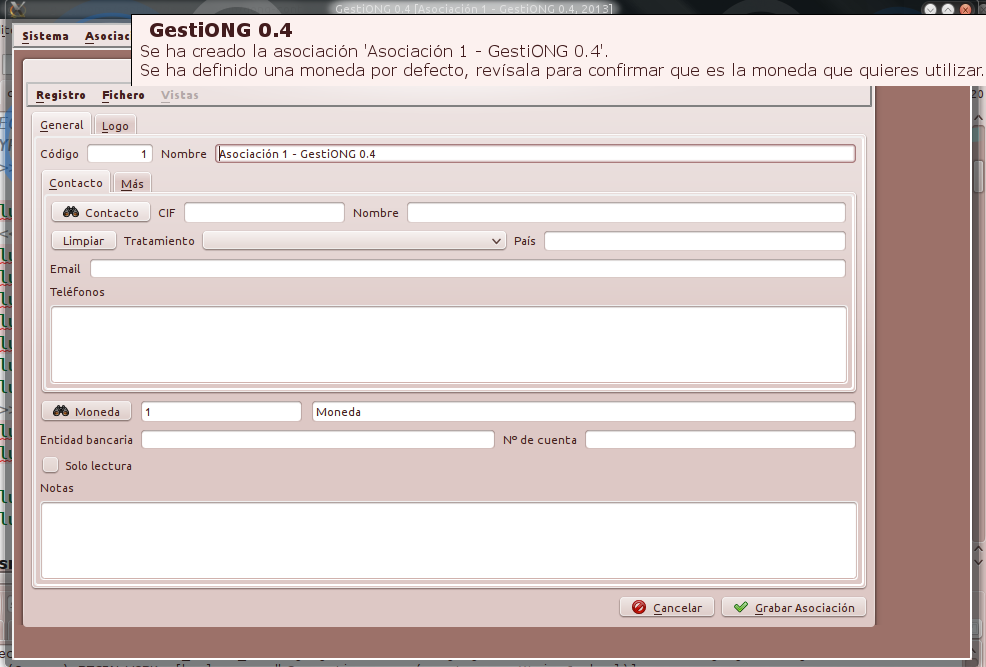
\includegraphics[width=\linewidth]{images/empresainicial.png}

\section{Datos importantes}

\begin{description}
 \item [Nombre] El nombre o razón social de la \organizacion. Puede utilizarse el nombre comercial o un nombre más conocido y más abajo, en el contacto, el nombre jurídico o legal de la \organizacion. Este nombre aparecerá más destacado en el encabezado de las facturas que emitamos. A modo de ejemplo, una persona en el régimen de autónomos introduciría el nombre comercial de su empresa aquí.
 \item [Contacto] Estos son los datos legales de contacto de la \organizacion o de su representante. Aquí introducimos el CIF y el nombre jurídico. A continuación rellenamos todos los datos de la localización de la empresa. Los datos mínimos a  rellenar para poder emitir facturas legales en España son: Nombre, CIF y la dirección completa (Dirección, Localidad y Provincia).
 \item [Moneda] La moneda principal de esta \organizacion. Se pueden definir más monedas y sus tasas de cambio con respecto a la moneda principal.
\end{description}


\section{Datos secundarios}
Cualquiera de los datos a continuación pueden aparecer en los documentos que imprimamos, sin embargo, no son fundamentales para el funcionamiento del programa.
\begin{description}
 \item [email, teléfonos, fax, página web, ...] 
 \item [Entidad bancaria y Nº de cuenta] Representan la entidad y los 20 dígitos de la cuenta bancaria principal de la empresa.
 \item [Logo] Se puede elegir una imagen que aparecerá en los encabezados de los documentos que se impriman.
 \item [Solo lectura] Esta casilla se marca si queremos que no se pueda realizar ninguna operación que cambie el estado de la empresa: compras, ventas, añadir o borrar clientes, etc. Es decir, solo se pueden visualizar datos, pero no se puede modificar nada.
\end{description}


\section{Monedas}

\appname permite trabajar con diferentes monedas, tanto oficiales como complementarias o sociales. Al crear la primera empresa, se crea una moneda por defecto a partir de los valores de la configuración de tu ordenador. Se pueden crear más monedas así como cambiar sus parámetros (por ejemplo, la tasa de cambio con respecto a la moneda principal) desde el menú \menu{Empresa->Moneda}.

\section{Tipos de IVA}

Se puede importar la definición de los tipos de IVA estándar con la opción \menu{Fichero=>Importar} del fichero de Tipos de IVA.

Buscar en la agencia tributaria: Nuevos tipos impositivos en el IVA

\url{http://www.agenciatributaria.es/AEAT.internet/Inicio_es_ES/_Segmentos_/Empresas_y_profesionales/Empresas/IVA/IVA.shtml}

\section{Formas de pago}

La definición de las formas de pago se realiza desde el menú \menu{Sistema->Formas de pago}. Se puede importar una lista predefinida de formas de pago con la opción \menu{Fichero->Importar}.

Formas de pago predefinidas:
\begin{enumerate}
 \item 
  \begin{description}
  \item [Contado] El documento (factura o albarán) se considera pagado por caja con la moneda principal en el mismo momento de ser emitido. No se generará ningún recibo.
  \end{description}
 \item
  \begin{description}
  \item [A reposición] El importe queda pendiente en el documento y se genera un recibo que será pagado en un momento posterior indefinido.
  \end{description}
\end{enumerate}

